%%%%%%%%%%%%%%%%%%%%%%%%%%%%%%%%%%%%%%%%%
% Presentazione tesi (10 minuti)
% Basata sul template Beamer fornito
%%%%%%%%%%%%%%%%%%%%%%%%%%%%%%%%%%%%%%%%%

\documentclass[
	11pt
]{beamer}

\usepackage[italian]{babel}
\usepackage{booktabs}
\usepackage{amsmath}
\usepackage{graphicx}
\usepackage{tikz}

% Tema coerente con il template
\usetheme{Madrid}
\usefonttheme{default}
\usepackage{palatino}
\usepackage[default]{opensans}
\useinnertheme{circles}

% Riduzione testo in footer e navigazione pulita
\setbeamertemplate{navigation symbols}{}
\setbeamertemplate{footline}[frame number]

% Info presentazione
\title[GoDP e Differential Privacy]{GoDP: una soluzione pratica per la Differential Privacy su dati sensibili}
\subtitle{Tesi magistrale in Ingegneria Informatica}
\author[Riccardo Barbieri]{Riccardo Barbieri}
\institute[UNIBO]{Alma Mater Studiorum -- Universita di Bologna \\ \smallskip Corso di Laurea Magistrale in Ingegneria Informatica}
\date[A.A. 2023/2024]{Relatore: Prof. Michele Colajanni \quad Correlatore: Ing. Silvio Russo \\ \smallskip Anno Accademico 2023/2024}

\begin{document}

%----------------------------------------------------------------------------------------
\begin{frame}
	\titlepage
\end{frame}

%----------------------------------------------------------------------------------------
\begin{frame}
	\frametitle{Struttura della presentazione}
	\begin{itemize}
		\item Problema e obiettivo
		\item Fondamenti DP: $\varepsilon$, $\delta$, budget
		\item GoDP: design e uso pratico
		\item Validazione: difference attack
		\item Risultati e conclusioni
	\end{itemize}
\end{frame}

%----------------------------------------------------------------------------------------
\begin{frame}
	\frametitle{Problema e obiettivo}
	\begin{block}{Problema}
		Anonimizzazione tradizionale fragile con informazioni ausiliarie.
	\end{block}

	\begin{block}{Obiettivo della tesi}
		Rendere la Differential Privacy applicabile in modo pratico su dataset piccoli/medi.
	\end{block}

	\begin{alertblock}{Contributo}
		\textbf{GoDP}: CLI in Go + specifica \textbf{DPYaml} per creare release aggregate DP.
	\end{alertblock}
\end{frame}

%----------------------------------------------------------------------------------------
\begin{frame}
	\frametitle{Differential Privacy in una slide}
	\begin{equation*}
		\Pr[\mathcal{M}(D_1) \in S] \le e^{\varepsilon}\Pr[\mathcal{M}(D_2) \in S] + \delta
	\end{equation*}

	\begin{itemize}
		\item $\varepsilon \downarrow$ $\Rightarrow$ maggiore privacy, minore utilita
		\item $\delta$: probabilita di eventi distintivi
	\end{itemize}

	\vspace{2mm}
	\centering
	\textbf{Trade-off centrale: privacy vs accuratezza}
\end{frame}

%----------------------------------------------------------------------------------------
\begin{frame}
	\frametitle{GoDP: architettura e flusso}
	\begin{columns}[t]
		\begin{column}{0.50\textwidth}
			\textbf{Input}
			\begin{itemize}
				\item CSV
				\item file DPYaml
			\end{itemize}

			\textbf{Motore}
			\begin{itemize}
				\item Apache Beam + Privacy on Beam
				\item Operazioni: count, sum, mean
				\item Filtri e tipi dichiarativi
			\end{itemize}
		\end{column}
		\begin{column}{0.48\textwidth}
			\textbf{Output}
			\begin{itemize}
				\item Aggregazioni DP
				\item Budget tracciato per operazione
			\end{itemize}

			\textbf{Utilità}
			\begin{itemize}
				\item Riduce barriera tecnica
				\item Estendibile con funzioni custom
			\end{itemize}
		\end{column}
	\end{columns}
\end{frame}

%----------------------------------------------------------------------------------------
\begin{frame}
	\frametitle{Threat model (modello centralizzato)}
	\begin{figure}
		
\includegraphics[width=0.88\linewidth]{../plots/centralized_dp_model.pdf}
	\end{figure}

	\centering
	\small Curatore fidato, analista/attaccante con informazioni ausiliarie.
\end{frame}

%----------------------------------------------------------------------------------------
\begin{frame}
	\frametitle{Difference attack: idea}
	\begin{figure}
		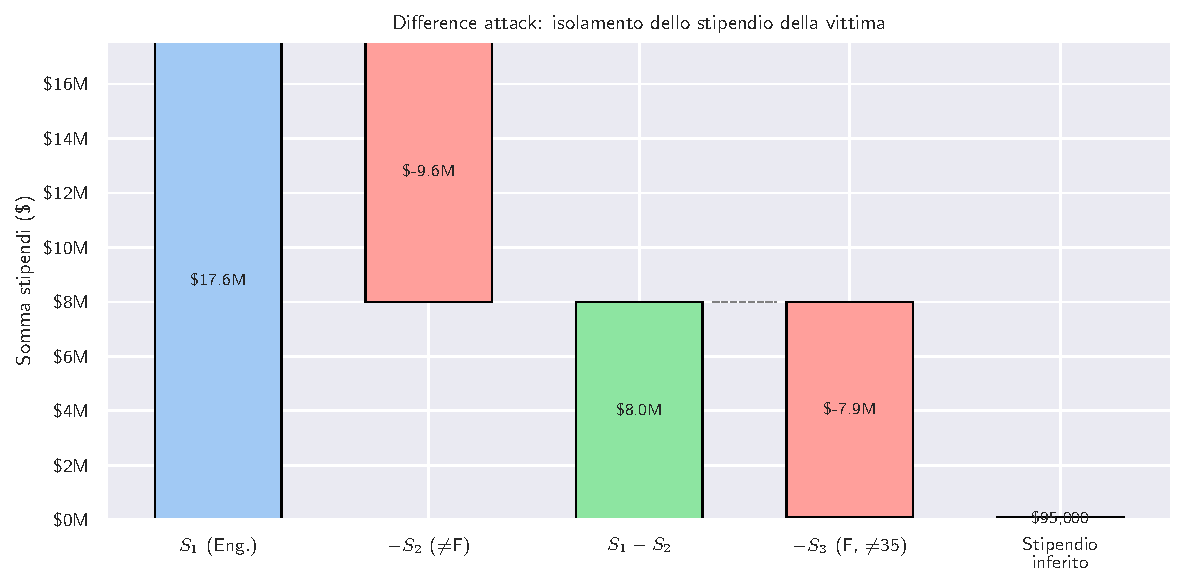
\includegraphics[width=0.80\linewidth]{../plots/difference_attack_waterfall.pdf}
	\end{figure}

	\centering
	\small Con query aggregate e sottrazioni successive si isola il contributo della vittima.
\end{frame}

%----------------------------------------------------------------------------------------
\begin{frame}
	\frametitle{Risultati principali dell'esperimento}
	\begin{figure}
		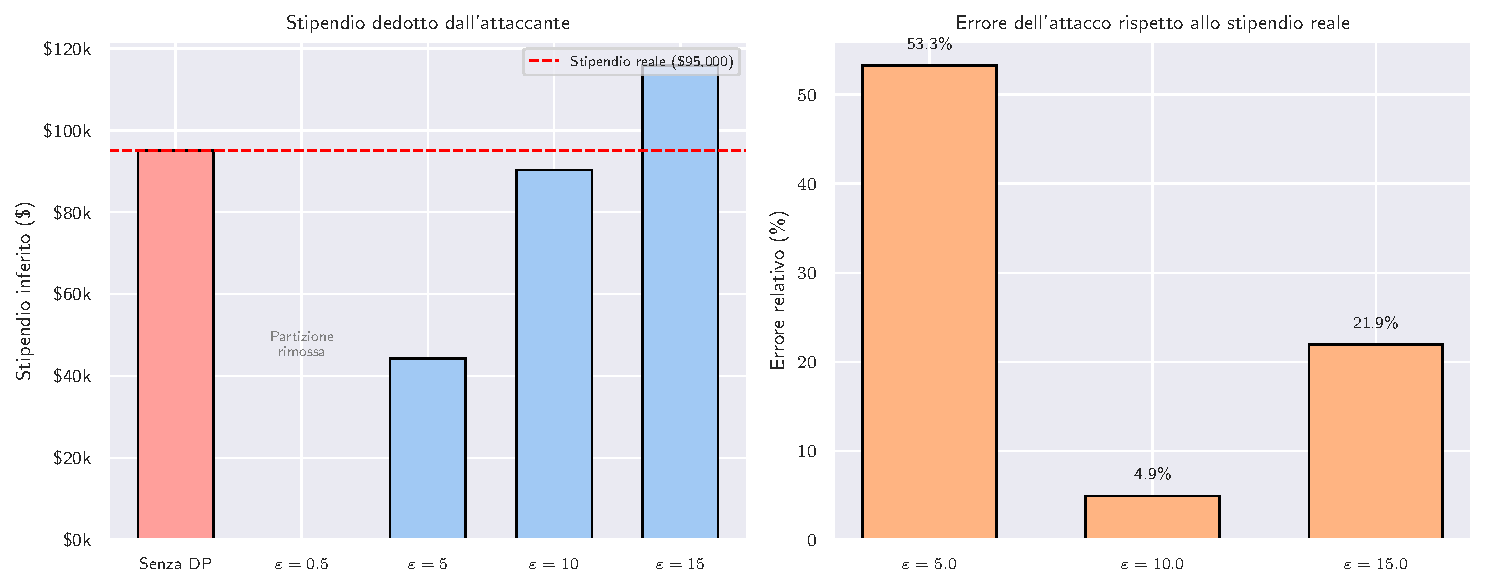
\includegraphics[width=0.95\linewidth]{../plots/attack_comparison.pdf}
	\end{figure}

	\vspace{-2mm}
	\begin{itemize}
		\item Senza DP: attacco riuscito (stipendio esatto)
		\item Con DP ($\varepsilon=0.5$): query critiche rimosse
		\item Con DP ($\varepsilon=5,10,15$): inferenza rumorosa, precisione ridotta
	\end{itemize}
\end{frame}

%----------------------------------------------------------------------------------------
\begin{frame}
	\frametitle{Rumore e scelta di $\varepsilon$}
	\begin{figure}
		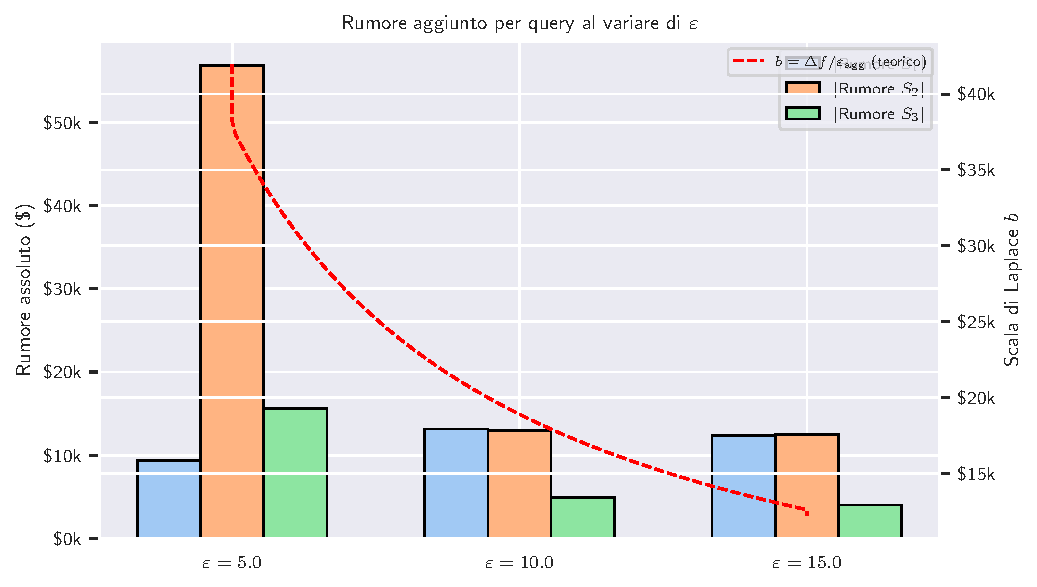
\includegraphics[width=0.92\linewidth]{../plots/noise_vs_epsilon.pdf}
	\end{figure}

	\vspace{-1mm}
	\begin{itemize}
		\item Scala teorica: $b = \Delta f / \varepsilon_{agg}$
		\item Nel difference attack il rumore si compone su 3 query
	\end{itemize}
\end{frame}

%----------------------------------------------------------------------------------------
\begin{frame}
	\frametitle{Conclusioni}
	\begin{itemize}
		\item GoDP rende la DP \textbf{usabile} in workflow reali
		\item L'esperimento conferma la protezione contro de-anonimizzazione
		\item La scelta di $\varepsilon$ resta \textbf{decisione di dominio}
	\end{itemize}

	\vspace{4mm}
	\begin{block}{Sviluppi futuri}
		Valutazione multi-run, supporto a scenari decentralizzati, estensione operazioni.
	\end{block}
\end{frame}

%----------------------------------------------------------------------------------------
\begin{frame}[plain]
	\begin{center}
		{\Huge Grazie per l'attenzione}
	\end{center}
\end{frame}

%----------------------------------------------------------------------------------------
\end{document}
